%*******************************************
\section{Evaluation}
%*******************************************
\label{s:evaluation}
\textbf{VLL FORMS IN APPENDIX? }As a final step the Anti-Phishing Education we have designed and implemented needs to be evaluated which is the goal of this chapter.
 The app will be evaluated with the aid of a user study.
 After introducing our study design, we will state our hypothesis and explain how we are going to measure our statements in order to prove that they are true or false.
 Finally, we will analyze our results and state our conclusion.


%===========================================
%\subsection{Participant Recruitment}
%===========================================
%Oder was soll hier rein? ;)
%osn - freundes freunde
%telefon -freundes freunde
%flyer ausgeteilt
%flyer per e-mail an sehr viele professoren geschickt und gebeten weiter an studenten zu leiten
%ein paar leute auf der straße angesprochen - da erfolglos
%Verlosung eines amazin gutscheins


%===========================================
\subsection{Study Design}
%===========================================
For time reasons and lack of participants we decided to run a "Before and After App" Study with the same groups of people.
 Specifically, our user study is structured as follows:

\begin{enumerate}
	\item \textbf{General Before-Survey} At the beginning the participants have to fill out a general survey, where they have to judge their own knowledge on the topic of Internet security in general.
 For instance, they are asked whether it is easy for them to distinguish legitimate e-mails and websites from fake ones.

	\item \textbf{Website-Survery Before} In this part of the user study the participants gets a list of screenshots of websites.
 The screenshots had been taken with the standard browser of an Android tablet.
 In total, the user is shown 16 screenshots, with 8 phishing and 8 valid URLs.
 The user has to decide whether he would enter confidential data on the shown website.
 Additionally, he has to encircle the part of the screenshot which was the primary reason for his decision.
 Then, the user has to indicate how sure he was about his answers on a Likert scale.
 Finally, the user is asked whether he knows the vendor of the website and whether he has a account there.

	\item \textbf{Play App} After the "Website-Survey Before" the users get the smartphones in order to play the app.
 To save time, we skipped the introduction 2 part ("access address bar") for the user study.
 The user has half an hour to play the app.
 After half an hour they are asked to put the smartphones aside.
 Then, we collect the smartphones and note the reached points in each level.

	\item \textbf{Website-Survery After} After playing the app, the participants get a second website-survey.
 In this, all examples of the previous survey are included.
 Moreover, it contains 8 further website screenshots of which 4 have phishing and the remaining 4 have valid URLs.

	\item \textbf{General After-Survey} Finally, the participants are asked to fill out a form with questions to their demographics.
 This form does also contain questions related to the SUS and some other questions regarding their impression of the app.



\end{enumerate}

%===========================================
\subsection{Hypotheses}
%===========================================
In order to evaluate the effectiveness and usability of our app we have formulated the following hypotheses for the user study:

\begin{enumerate}
	\item \textbf{Hypothesis 1 - Mistakes} After playing the app, the users make significantly less mistakes in detecting phishing websites compared to before playing the app.

	\item \textbf{Hypothesis 2 - URL Based Decision} After playing the app, the users base their primary decision on whether a website is a phishing website or not significantly more often based on the URL compared to before playing the app.

	\item \textbf{Hypothesis 3 - URL Comprehension} After playing the app the user understands the importance of the second- and top-level domain of a URL as the only criteria to detect phishing websites.

	\item \textbf{Hypothesis 4 - Good Usability} The app is easy to understand and to use.

\end{enumerate}


%===========================================
\subsection{Measurement}
%===========================================
In the following we will elaborate on how we are going to measure the statements of our hypothesis and show that they are true or false.


\begin{enumerate}
	\item \textbf{Hypothesis 1 - Mistakes} Correct answers in "Website-Survery After" $>>$ correct answers in "Website-Survery Before" 
	\item \textbf{Hypothesis 2 - URL Based Decision} Number of URL markings in "Website-Survery After" $>>$ number of URL markings in "Website-Survery Before" 
	\item \textbf{Hypothesis 3 - URL Comprehension} Number of marked second- and/or top-level domains of URLs in "Website-Survery After"  $>>$ number of marked second- and/or top-level domains of URLs in "Website-Survery Before" 
	\item \textbf{Hypothesis 4 - Good Usability} System Usability Scale (SUS) $>$ 68
\end{enumerate}

%===========================================
\subsection{Results and Analysis}
%===========================================
\subsection{Analysis of our hypotheses}
\label{s:hypanalysis}

\begin{figure}
\centering
\subfigure[Before]{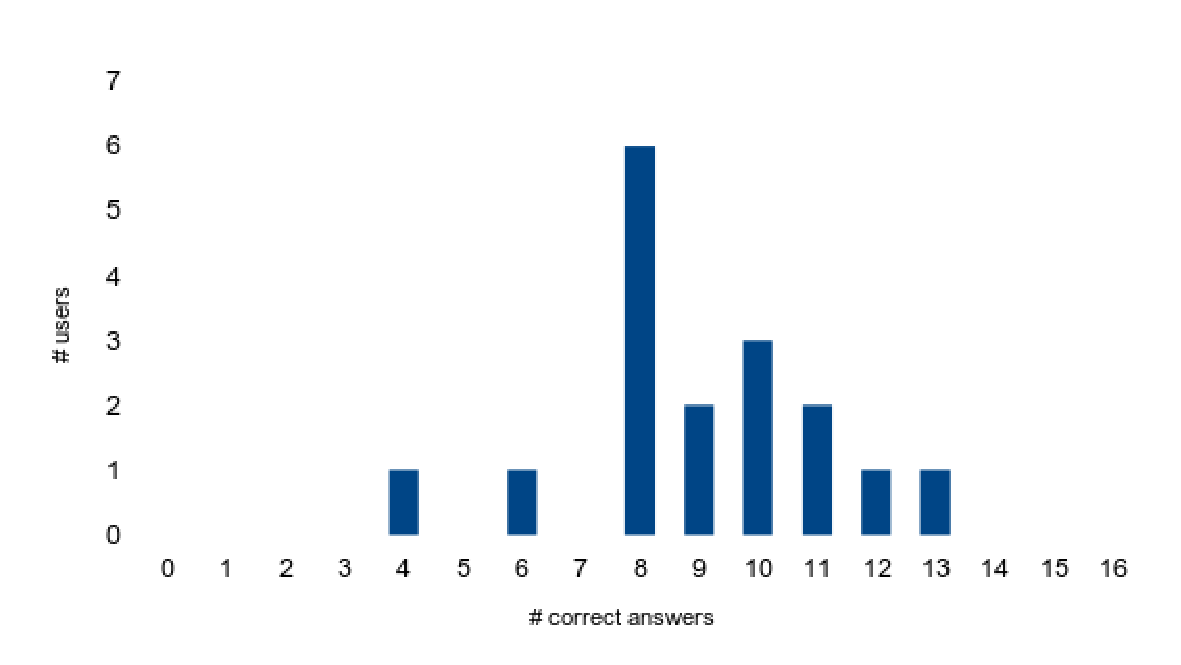
\includegraphics[width=0.45\textwidth]{graphix/hyp1b.pdf}}
\subfigure[After (all URLs)]{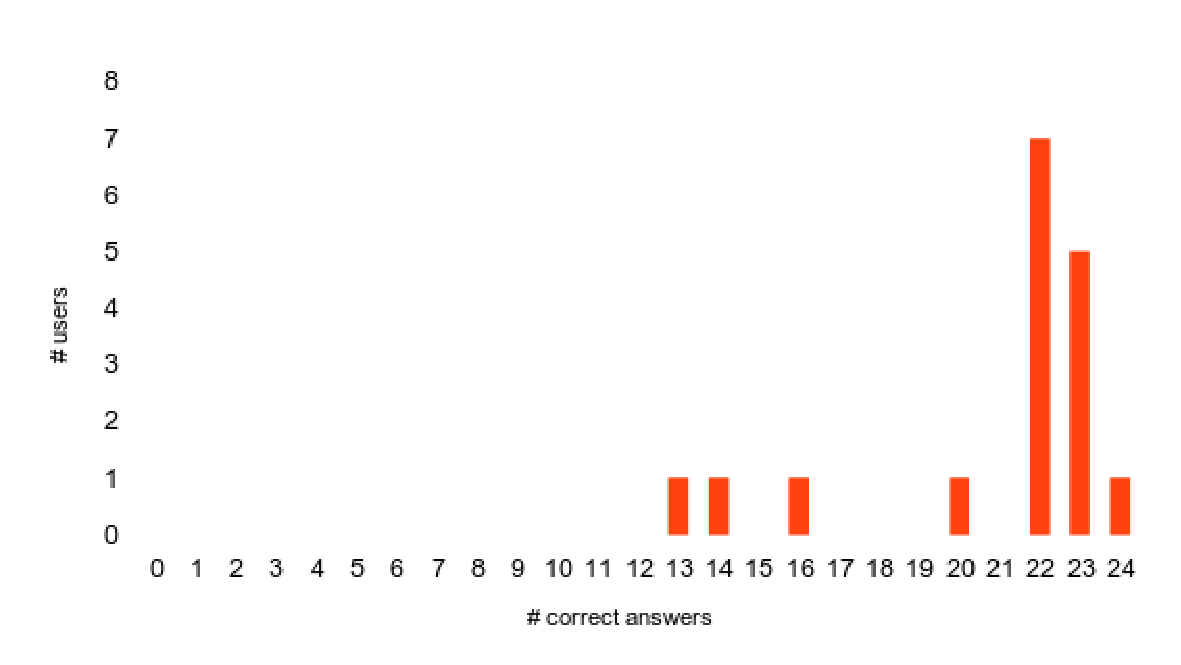
\includegraphics[width=0.45\textwidth]{graphix/hyp1a.pdf}}
\subfigure[After (New URLs)]{\label{fig:hyp1resultsanew}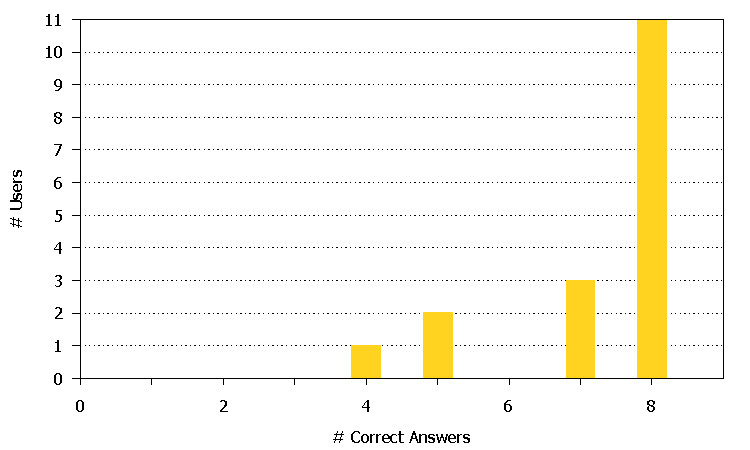
\includegraphics[width=0.45\textwidth]{graphix/hyp1anew.pdf}}
\subfigure[After (Repeated URLs)]{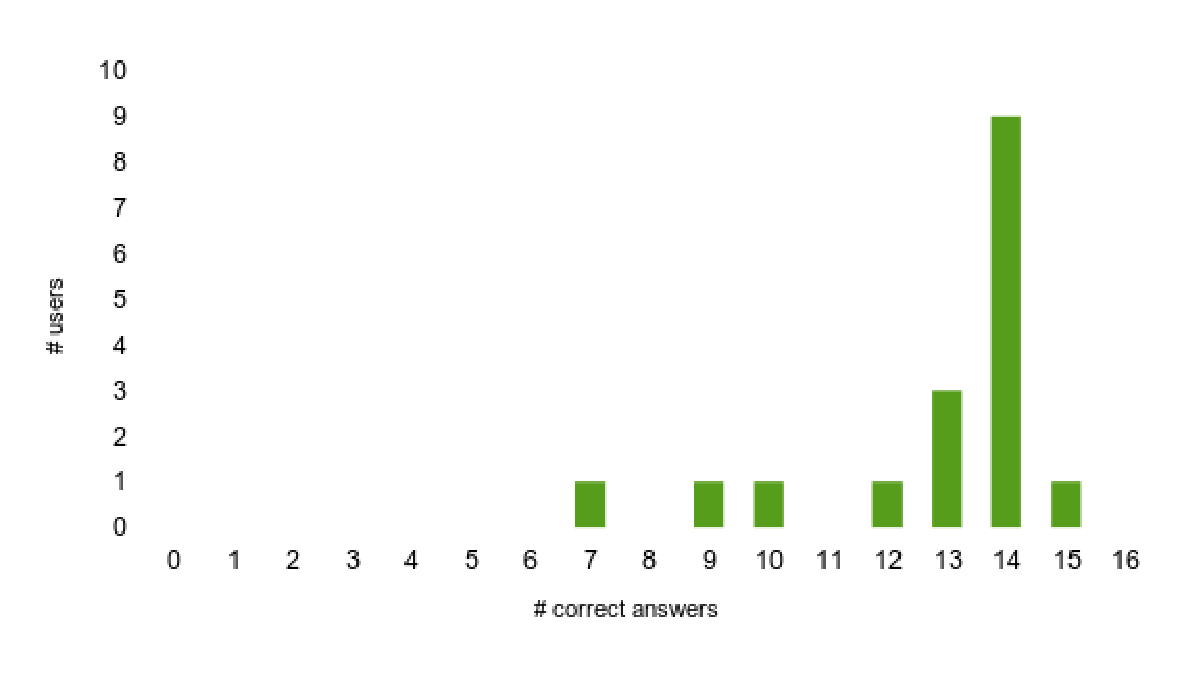
\includegraphics[width=0.45\textwidth]{graphix/hyp1arepeat.pdf}}
\caption{Correct Answers}
\label{fig:hyp1results}
\end{figure}

\begin{figure}
\centering
\subfigure[Before]{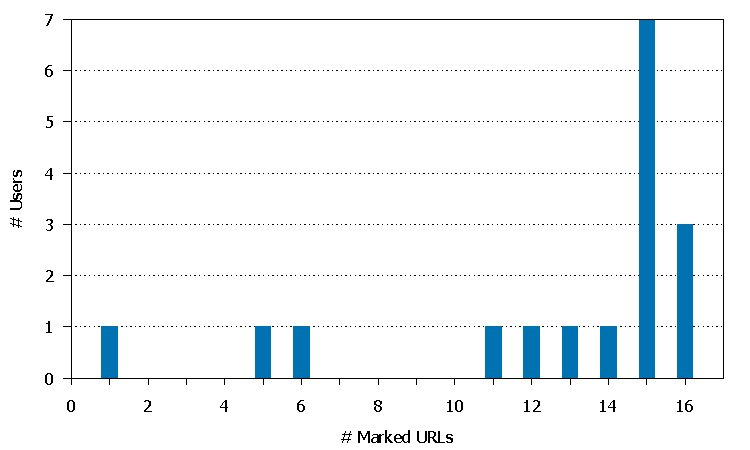
\includegraphics[width=0.45\textwidth]{graphix/hyp2b.pdf}}
\subfigure[After]{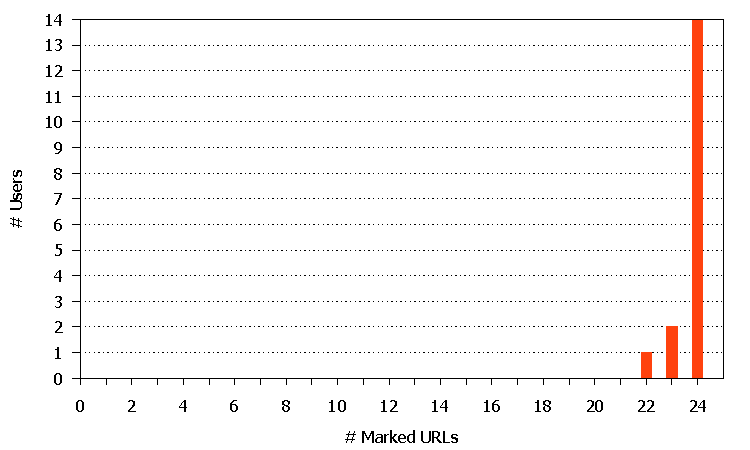
\includegraphics[width=0.45\textwidth]{graphix/hyp2a.pdf}}
\caption{URL marked}
\label{fig:hyp2results}
\end{figure}

\begin{figure}
\centering
\subfigure[Before]{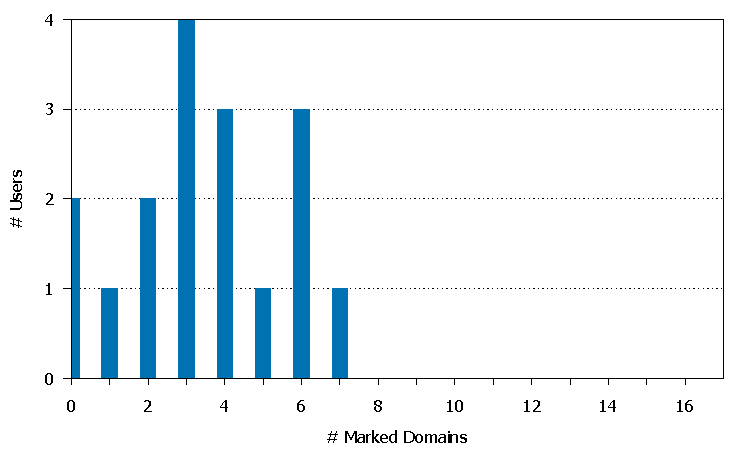
\includegraphics[width=0.45\textwidth]{graphix/hyp3b.pdf}}
\subfigure[After]{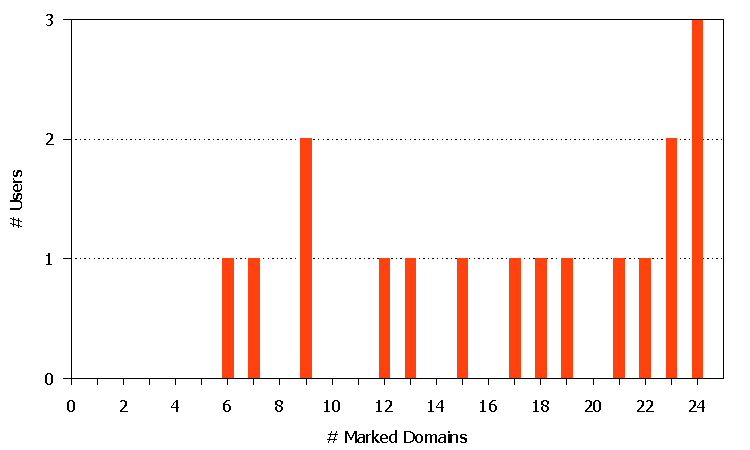
\includegraphics[width=0.45\textwidth]{graphix/hyp3a.pdf}}
\caption{Domain marked}
\label{fig:hyp3results}
\end{figure}

\begin{description}
\item[Hypothesis 1]
\autoref{fig:hyp1results} shows the reslts of our study according to hypothesis 1. One can clearly see that the majority of the users identified more URLS correctly after using the app than before. While most participants correctly identified 8 out of 16, i.e. 50\%, websites before they played the app, the majority gave correct answers to 22 out of 24 websites afterwards, i.e. 91.67\%. One could argue that this increase is based on the fact that the examples are mainly the same. \autoref{fig:hyp1resultsanew} however shows that the user also got most of the new URLs right. Therefore we assume that we can furthermore ignore this learning effect. 
\item[Hypothesis 2]
\autoref{fig:hyp2results} shows how many users marked the URL as their main source of decision. Most of the users already based most of their decisions on the URL before. Occasionally users marked the content or the padlock. However only 3 Users (17.65\%) always marked the URL. Afterwards we see that most users (82.35\%) always based the decision on the URL and only 3 Users made on or two mistakes.
\item[Hypothesis 3]
\item[Hypothesis 4]
\end{description}

\subsubsection{Further exploration}
Some of the results can not be proven statistically.
Mainly because of the low sample count. 
Therefore we will only exploratorily analyze these results.
\begin{description}
\item[text]
\end{description}
%===========================================
\subsection{Discussion}
%===========================================
%===========================================
\subsection{Conclusion}
%===========================================
